\section{A programming model for packet scheduling}
\label{s:pifo}

For work-conserving scheduling algorithms, the characteristic feature
is the order in which packets are scheduled; for non-work-conserving
ones, it is the time at which each packet is sent. Moreover, for most
algorithms used in practice, these two decisions can be determined
definitively when a packet is enqueued into the packet
buffer~\cite{pifo_hotnets}.

Our programming model is built around this observation and has two
underlying components:
\begin{CompactEnumerate}
\item The {\em push-in first-out queue (PIFO)}~\cite{pifo}, which
  maintains the scheduling order or scheduling time for enqueued
  elements. A PIFO is a priority queue that allows elements to be
  enqueued into an arbitrary position based on the element's {\em
    rank}, but dequeues elements from the head. Elements with a lower
  rank are dequeued first; if two elements have the same value, the
  element enqueued earlier is dequeued first.

\item The computation of an element's rank before it is enqueued into
  a PIFO. We model this computation as a {\em packet
    transaction}~\cite{domino_sigcomm}, an atomically executed block
  of code that is executed once for each element before enqueuing it
  in a PIFO.\footnote{Any state visible on the switch after processing
    $N$ consecutive packets is identical to a serial execution of the
    transactions across the $N$ packets in order of packet
    arrival~\cite{domino_sigcomm}.}
\end{CompactEnumerate}

We note that scheduling with the PIFO abstraction does not require packets to be
stored in per-flow queues.

\begin{figure}
\begin{lstlisting}[style=customc]
f = flow(p) # compute flow from packet p
if f in last_finish:
 p.start = max(virtual_time, last_finish[f])
else: # p is first packet in f
 p.start = virtual_time
last_finish[f] = p.start + p.length/f.weight
p.rank = p.start
\end{lstlisting}
\caption{Scheduling transaction for STFQ. {\tt p.x} refers to a packet
  field {\tt x} in packet {\tt p}.  {\tt y} refers to a state variable
  that is persisted on the switch across packets, e.g., {\tt last\_finish}
  and {\tt virtual\_time} in this snippet. {\tt p.rank} denotes the
  packet's computed rank.}
\label{fig:sched_trans}
\end{figure}

%%% Figure for HPFQ below %%%
\begin{figure*}
\begin{subfigure}[b]{.2\textwidth}
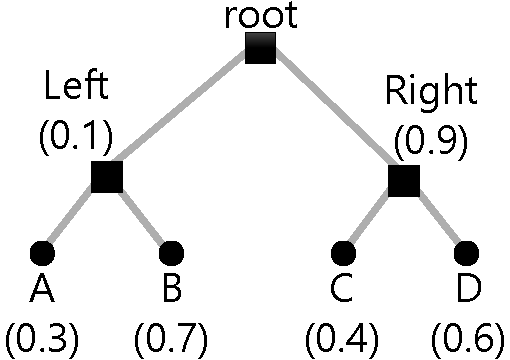
\includegraphics[width=\textwidth]{pifo_hpfq_example.pdf}
\caption{Algorithm}
\label{fig:hpfq_algo}
\end{subfigure}
\vrule
\begin{subfigure}[b]{.3\textwidth}
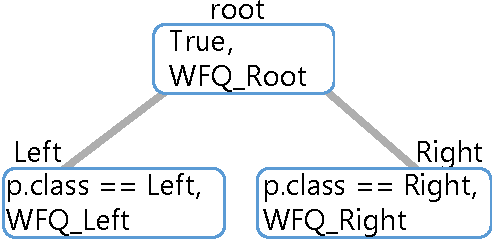
\includegraphics[width=\textwidth]{pifo_hpfq_program.pdf}
\caption{Scheduling tree}
\label{fig:hpfq_tree}
\end{subfigure}
\vrule
\begin{subfigure}[b]{.5\textwidth}
\begin{lstlisting}[style=customc]
f = flow(p) # see caption below
if f in last_finish:
  p.start = max(virtual_time, last_finish[f])
else:
  p.start = virtual_time
last_finish[f] = p.start + p.length / f.weight
p.rank = p.start
\end{lstlisting}
\caption{Scheduling transaction for WFQ\_Root, WFQ\_Left, and
  WFQ\_Right.}
\label{fig:hpfq_trans}
\end{subfigure}
\caption{Programming HPFQ using PIFOs. ``Left'' and ``Right'' are
  classes. A, B, C, and D are flows.  Within each tree node in the scheduling tree, the first
  line is the packet predicate and the second is the scheduling
  transaction. All three nodes execute the same code for the scheduling
  transaction except for their flow() function, which returns a packet's flow/class. For
  WFQ\_Root, it returns the packet's class: Left/Right. For WFQ\_Left
  and WFQ\_Right, it returns the packet's flow: A/B or C/D.}
\label{fig:hpfq}
\end{figure*}

We now describe the three main abstractions in our programming model. First, we
show how to use a {\em scheduling transaction} to program simple
work-conserving scheduling algorithms using a single PIFO~(\S\ref{ss:wfq}).
Second, we generalize to a {\em scheduling tree} to program hierarchical
work-conserving scheduling algorithms~(\S\ref{ss:hpfq}). Third, we augment
nodes of this tree with a {\em shaping transaction} to program
non-work-conserving scheduling algorithms~(\S\ref{ss:hshaping}).

\subsection{Scheduling transactions}
\label{ss:wfq}

A {\em scheduling transaction} is a block of code associated with a
PIFO that is executed once for each packet before the packet is
enqueued. The scheduling transaction computes the packet's rank, which
determines its position in the PIFO.  
%Scheduling transactions can be used to program work-conserving
%scheduling algorithms. In particular,
A single scheduling transaction and PIFO are sufficient to specify any
scheduling algorithm where the relative scheduling order of packets
already in the buffer does not change with the arrival of future
packets.

Weighted Fair Queueing (WFQ)~\cite{wfq} is one example. It achieves weighted
max-min allocation of link capacity across flows\footnote{In this paper, a flow is any set of packets sharing
common values for specific packet fields.} sharing a link.  Approximations to
WFQ\footnote{\an{An approximation is required because the original WFQ
algorithm~\cite{wfq} has a complex virtual time calculation.}} include Deficit
Round Robin (DRR)~\cite{drr}, Stochastic Fairness Queueing (SFQ)~\cite{sfq},
and Start-Time Fair Queueing (STFQ)~\cite{stfq}. We consider STFQ here, and
show how to program it using the scheduling transaction in
Figure~\ref{fig:sched_trans}.

%\footnote {STFQ is identical to the
%  original WFQ algorithm~\cite{wfq}, but has a more practical virtual
%  time calculation.}

%Getting rid of the footnote on WFQ.
%%\footnote {\an{An approximation is required because the original
%%WFQ algorithm~\cite{wfq} has a complex virtual time calculation.}}

Before a packet is enqueued, STFQ computes a {\em virtual start time}
for that packet (\texttt{p.start} in Figure~\ref{fig:sched_trans}) as
the maximum of the {\em virtual finish time} of the previous packet in
that packet's flow (\texttt{last\_finish[f]} in
Figure~\ref{fig:sched_trans}) and the current value of the {\em
  virtual time} (\texttt{virtual\_time} in Figure~\ref{fig:sched_trans}), a state variable that tracks the virtual
start time of the last dequeued packet across all flows
(\S\ref{ss:add_impl} discusses how this state variable can be accessed
on enqueue). Packets are scheduled in order of increasing virtual
start times, which is the packet's rank in the PIFO.

\subsection{Scheduling trees}
\label{ss:hpfq}

Scheduling algorithms that require changing the relative order of
buffered packets when a new packet arrives cannot be programmed using
a single scheduling transaction and PIFO. An important class of such
algorithms are {\em hierarchical} schedulers that compose multiple
scheduling policies at different levels of the hierarchy. We introduce
a {\em scheduling tree} for such algorithms.

To illustrate a scheduling tree, consider Hierarchical Packet Fair
Queueing (HPFQ)~\cite{hpfq}. HPFQ first divides link capacity between
classes, then recursively between sub classes in each class, all the
way down to the leaf nodes.  Figure~\ref{fig:hpfq_algo} provides an
example; the number on each child indicates its weight relative to its
siblings.  HPFQ cannot be realized using a single scheduling
transaction and PIFO because the relative scheduling order of packets
that are already buffered can change with future packet arrivals
(Section 2.2 of the HPFQ paper~\cite{hpfq} provides an example).

%\hb{Can we
%  provide the example here?}
% I think it distracts from the overall flow. Also don't want to repeat
% something that can be looked up.

HPFQ {\em can}, however, be realized using a tree of PIFOs, with a
scheduling transaction attached to each PIFO in the tree. To see how,
observe that HPFQ executes WFQ at each level of the hierarchy, with
each node using WFQ among its children. As discussed in
\S\ref{ss:wfq}, a single PIFO encodes the current scheduling order for
WFQ, i.e., the scheduling order if there are no further
arrivals. Similarly, a tree of PIFOs (Figure~\ref{fig:pifo_encoding}),
where each PIFO's elements are either packets or references to other
PIFOs, can be used to encode the current scheduling order of HPFQ and
other hierarchical scheduling algorithms. To determine this scheduling
order, inspect the root PIFO to determine the next child PIFO to
schedule. Then, recursively inspect the child PIFO to determine the
next grandchild PIFO to schedule, until reaching a leaf PIFO that
determines the next packet to schedule.
%Figure~\ref{fig:pifo_encoding} shows this encoding.

%PIFO encoding figure
\begin{figure}
\centering
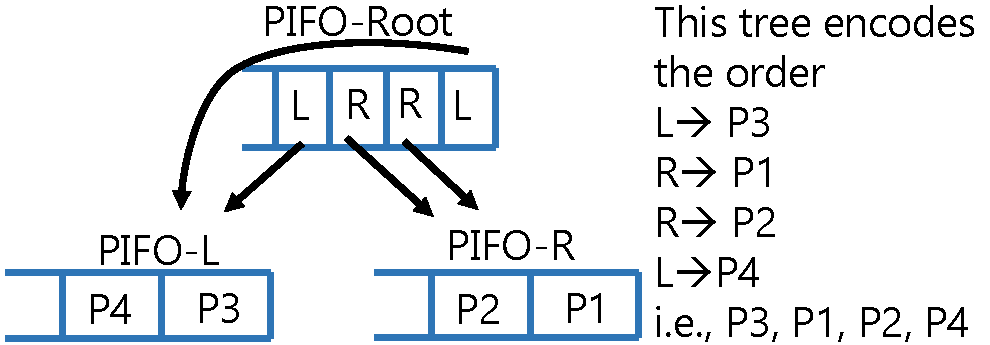
\includegraphics[width=0.45\textwidth]{pifo_pifo_tree_encoding.pdf}
\caption{PIFO trees encode current scheduling order.}
\label{fig:pifo_encoding}
\end{figure}


The current scheduling order of the PIFO tree can be modified as
packets are enqueued, by executing a scheduling transaction at each
node in the PIFO tree. This is our second programming abstraction: a
{\em scheduling tree}.  Each node in this tree is a tuple with two
attributes. First, a packet predicate that specifies which packets
execute that node's scheduling transaction before enqueuing an
element into that node's PIFO; this element is either a packet or a
reference to a child PIFO of the node.  Second, a scheduling
transaction that specifies how the rank is computed for elements
(packet or PIFO references) that are enqueued into the node's
PIFO. Figure~\ref{fig:hpfq_tree} shows an example for HPFQ.

When a packet is enqueued into a scheduling tree, it executes one
transaction at each node whose packet predicate matches the arriving
packet. These nodes form a path from a leaf to the root of the tree
and the transaction at each node on this path updates the scheduling
order at that node. One element is enqueued into the PIFO at each node
on the path from the leaf to the root. At the leaf node, that element
is the packet itself; at the other nodes, it is a reference to the
next PIFO on the path towards the leaf. Packets are dequeued in the
order encoded by the tree of PIFOs~(Figure~\ref{fig:pifo_encoding}).

\subsection{Shaping transactions}
\label{ss:hshaping}

%%% Figure for hshaping below %%%
\begin{figure*}
\begin{subfigure}[b]{0.2\textwidth}
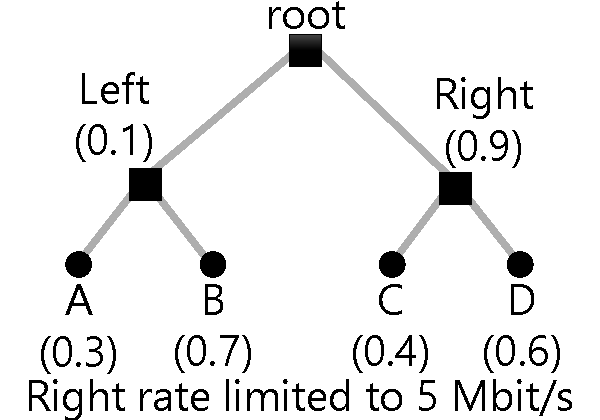
\includegraphics[width=\textwidth]{pifo_hshaping_example.pdf}
\caption{Algorithm}
\label{fig:hshaping_algo}
\end{subfigure}
\vrule
\begin{subfigure}[b]{0.3\textwidth}
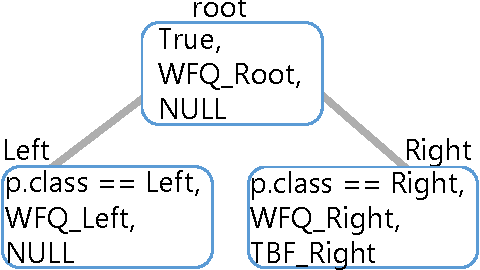
\includegraphics[width=\textwidth]{pifo_hshaping_program.pdf}
\caption{Scheduling tree}
\label{fig:hshaping_tree}
\end{subfigure}
\vrule
\begin{subfigure}[b]{0.5\textwidth}
\begin{lstlisting}[style=customc]
tokens = tokens + r * (now - last_time)
if (tokens > B):
  tokens = B
if (p.length <= tokens):
  p.send_time = now
else:
  p.send_time = now + (p.length - tokens) / r
tokens = tokens - p.length
last_time = now
p.rank = p.send_time
\end{lstlisting}
\caption{Shaping transaction for TBF\_Right.}
\label{fig:hshaping_shaping_trans}
\end{subfigure}
\caption{Programming Hierarchies with Shaping using PIFOs. The third line
within each tree node in the scheduling tree is the shaping transaction. The scheduling
transactions for WFQ\_Right, WFQ\_Left, and WFQ\_Root are identical to
Figure~\ref{fig:hpfq}.}
\label{fig:hshaping}
\end{figure*}

So far, we have only considered work-conserving scheduling
algorithms. {\em Shaping transactions} allow us to program
non-work-conserving scheduling algorithms. Non-work-conserving
algorithms differ from work-conserving algorithms in that they decide
the {\em time} at which packets are scheduled as opposed to the
scheduling {\em order}. As an example, consider the algorithm shown in
Figure~\ref{fig:hshaping_algo}, which extends the previous HPFQ
example with the requirement that the Right class be limited to
5~Mbit/s. We refer to this example throughout the paper as {\em
  Hierarchies with Shaping}.

% Consider removing:
% Non-work-conserving algorithms
% differ from work-conserving algorithms in that they decide the {\em time} at
% which packets are scheduled as opposed to the scheduling {\em order}. 

To motivate our abstraction for non-work-conserving algorithms, recall
that a PIFO tree encodes the current scheduling order, by walking down
the tree from the root PIFO to a leaf PIFO to schedule packets.  With
this encoding, a PIFO reference can be scheduled
only if it resides in a PIFO and there is a chain of PIFO references
from the root PIFO to that PIFO reference. To program non-work-conserving
scheduling algorithms, we provide the ability to {\em defer} when a
PIFO reference is enqueued into the PIFO tree, and hence is
available for scheduling.

To defer enqueues into the PIFO tree, we augment nodes of the
scheduling tree with an optional third attribute: a {\em shaping
  transaction} that is executed on all packets matched by the node's
packet predicate. The shaping transaction on a node determines when a
reference to the node's PIFO is available for scheduling in the node's
{\em parent's} PIFO. The shaping transaction is implemented using a
{\em shaping PIFO} at the child---distinct from the scheduling PIFO at
all nodes---that holds references to the child's scheduling PIFO until
they are released to the parent's scheduling PIFO.  The shaping
transaction uses the wall-clock departure time as the rank for the
shaping PIFO, unlike the scheduling transaction that uses the relative
scheduling order as the rank.

Once a reference to the child's scheduling PIFO has been released to
the parent's scheduling PIFO from the child's shaping PIFO, it is
scheduled by executing the parent's scheduling transaction and
enqueuing it in the parent's scheduling PIFO. If a node has no shaping
transaction, references to that node's scheduling PIFO are
immediately enqueued into its parent's scheduling PIFO with no deferral.
The dequeue logic during shaping still follows Figure~\ref{fig:pifo_encoding}:
dequeue recursively from the root until we schedule a packet.

%\S\ref{ss:time_sequence} describes the timing of these operations.

%Anirudh->Mohammad; I think we are complicating things by repeatedly saying packet (or PIFO
%reference) It's correct to just say PIFO reference and forget about packets altogether.
% It makes for simpler semantics as well.
% It just mandates that even rate limiting a single flow will now need three PIFOs, as given below, but that's fine
% Child: shaping PIFO releases references to Child's scheduling PIFO to parent
% Child: scheduling PIFO holds packets.
% Parent's scheduling PIFO executes FIFO across references of Child's scheduling PIFO.
% This is a complicated way of implementing shaping at one level, but it simplifies semantics
% because only PIFO references can now be enqueue into the parent's scheduling PIFO, not packets.

Figure~\ref{fig:hshaping_shaping_trans} shows an example of a shaping
transaction that defers enqueues based on a Token Bucket Filter (TBF)
with a rate-limit of $r$ and a burst allowance $B$. Here, the packet's
wall clock departure time ({\tt p.send\_time}), is used as its rank in
the shaping PIFO. Figure~\ref{fig:hshaping_tree} shows how to use this
shaping transaction to program Hierarchies with Shaping: the TBF
shaping transaction (TBF\_Right) determines when PIFO references for
Right's scheduling PIFO are released to Root's scheduling PIFO.

\begin{figure}[!t]
  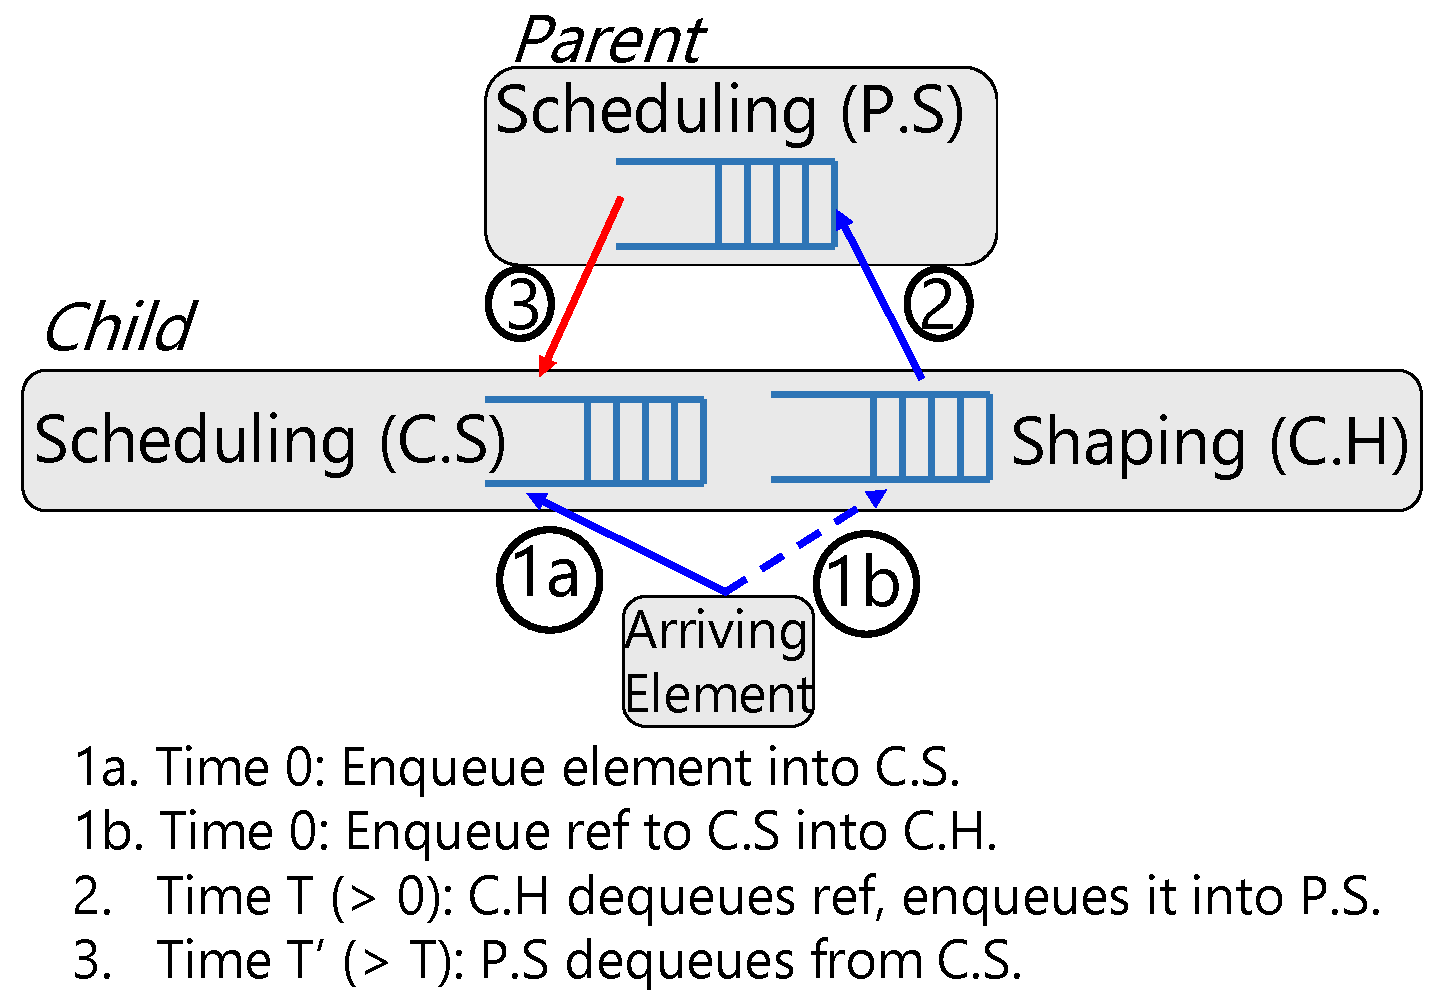
\includegraphics[width=\columnwidth]{pifo_shaping_semantics.pdf}
  \caption{\textit{Child's} shaping transaction (1b) {\em defers} enqueue
  into \textit{Parent's} scheduling PIFO (2) until time T.  Blue arrows
  show enqueue paths. Red arrows show dequeue paths.  }
  \label{fig:shaping_trans}
\end{figure}

\medskip
\noindent
\textbf{Timing of operations during shaping.}
When a packet is enqueued in a tree of PIFOs, it executes a scheduling
transaction at the leaf node whose predicate matches this packet.  It
then continues upward towards the root executing scheduling
transactions along the path, until it reaches the first node that also
has a shaping transaction attached to
it. Figure~\ref{fig:shaping_trans} shows the operations that occur at
this node, {\em Child}, and its parent, {\em Parent}, to implement
shaping.

Two transactions are executed at {\em Child}: the original scheduling
transaction to push an element into {\em Child}'s scheduling PIFO (step 1a
in Figure~\ref{fig:shaping_trans}) and a shaping transaction to push an
element $R$ (step 1b), which is a reference to {\em Child}'s scheduling
PIFO, into {\em Child}'s shaping PIFO. After $R$ is pushed into {\em Child}'s
shaping PIFO, further transactions for this packet are suspended until
$R$'s rank, the wall-clock time $T$, is reached.

At $T$, $R$ will be dequeued from {\em Child}'s shaping PIFO and
enqueued into {\em Parent}'s scheduling PIFO (step 2), making it available
for scheduling at {\em Parent}. The rest of the packet's path to the root is now
resumed starting at {\em Parent}. This suspend-resume process can occur
multiple times if there are multiple nodes with shaping transactions
along a packet's path from its leaf to the root.
